\section{Discussion and Conclusions}
	
	\begin{itemize}
		\item To include a detailed description of the physics behind the best fit model
		\item To refer to the original publications containing the XSPEC model components where the physics is described
		\begin{itemize}
			\item For \texttt{TBabs}: Wilms et al. \url{https://iopscience.iop.org/article/10.1086/317016/pdf}
			
			Now \texttt{phabs}
			\item For \texttt{ismabs}: Gatuzz et al. \url{https://iopscience.iop.org/article/10.1088/0004-637X/800/1/29/pdf}
			\item For \texttt{edge}: \url{https://heasarc.gsfc.nasa.gov/xanadu/xspec/manual/node247.html}
			\item For \texttt{rauch}: \url{http://astro.uni-tuebingen.de/~rauch/TMAF/TMAF.html}
		\end{itemize}
	\end{itemize}
	An inspection of the distribution of the residual suggests an approximately normal distribution, which can be observed in the best-fit models for all the observations, further supporting the validity of the model fit with values of $1<\chi^2_\text{red}<2$. Such a distribution of the residuals is displayed in figure \ref{fig:pn:resid-hist} for the observations of the EPIC-pn data.
	
	\begin{figure*}[!htb]
        \centering
        \begin{subfigure}[b]{0.51\textwidth}
            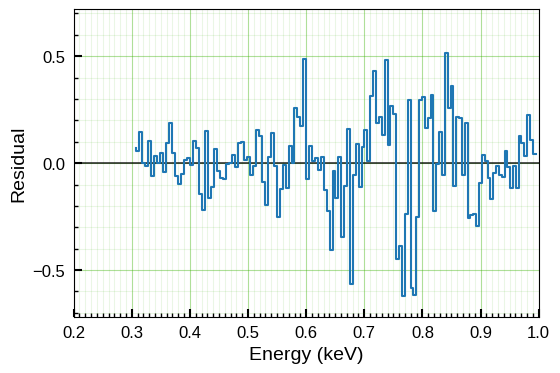
\includegraphics[width=\textwidth]{figures/resid/mr-vel-0111150101-pn_resid.png}
            \caption{Residuals between data and best-fit model for EPIC-pn observations}
            \label{fig:pn:resid}
        \end{subfigure}
        \hfill
        \begin{subfigure}[b]{0.39\textwidth}
            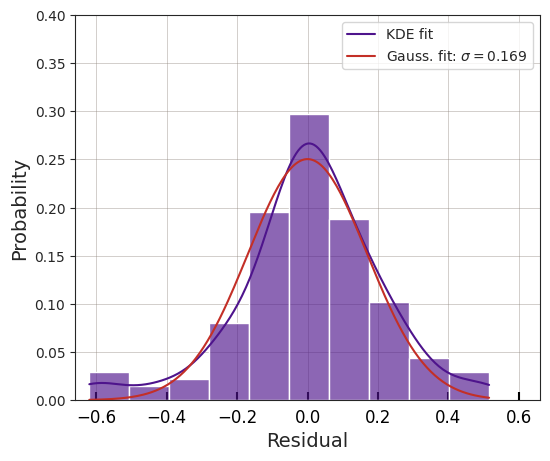
\includegraphics[width=\textwidth]{figures/resid/mr-vel-0111150101-pn_resid-hist.png}
	        \caption{Distribution of residuals from the best-fit model to EPIC-pn observations, along with the KDE function and fitted Gaussian}
	        \label{fig:pn:resid-hist}
        \end{subfigure}
        \caption{Residual statistics from best-fit model to all observations}
        \label{fig:all-obs:resid-stats}
    \end{figure*}
    
    As it can be seen in figure \ref{fig:pn:resid-hist}, the kernel density estimate (KDE) function of the distribution closely approximates a normal distribution centred about zero (zero indicating a perfect fit) and with a standard deviation of 0.169, thereby indicating that the observed count rate data can be considered to be random fluctuations which are normally distributed about the best-fit model.
    
    \begin{figure}[!htb]
    	\centering
    	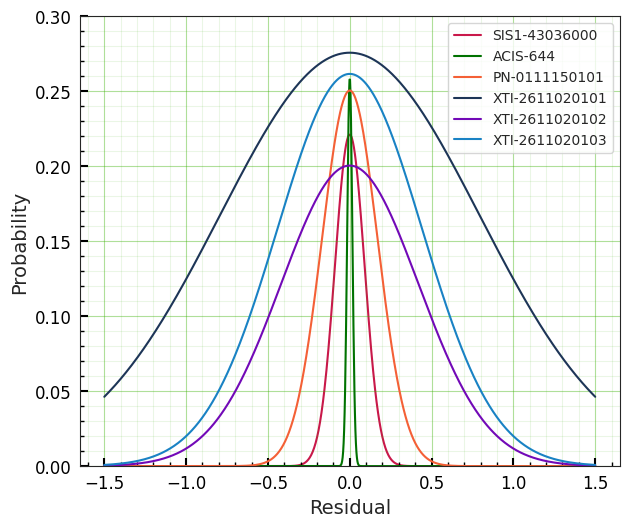
\includegraphics[width=0.45\textwidth]{figures/resid/mr-vel-resid-gaussfit_all-obs.png}
    	\caption{Gaussian approximations of the KDE functions for residual distributions of all observations}
    	\label{fig:all-obs:resid-gaussfit}
    \end{figure}
    
    In figure \ref{fig:all-obs:resid-gaussfit}, we find the Gaussian distribution fitted to all the observations. This figure shows that the quality of the fit is the best for the earlier Chandra, XMM-Newton and ASCA observations. For the recent NICER observations, the residuals show a wider spread spread about the perfect fit.